\chapter{Design} % (fold)
\label{cha:design}
Now that the problems are clear, it is time to present the system that should solve these problems: the SnoozZz system. This chapter describes the design of the system. This chapter is divided in to two parts: the components, that make up the system, and their responsibilities are listed in the first part; and the second part contains an overview of the components and how these work together.

\section{Components} % (fold)
\label{sec:components}
To setup the system, a few things are required. The first component is an accelerometer with some processing capability. The second component is a server to do the detection of the current sleep phase according to the data received from the server. A connection between the accelerometer and the server is required to transport data between the two components.
\subsection{Sensor} % (fold)
\label{sub:sensor}
The sensor used in the system is an accelerometer. This sensor monitors the x, y and z movement.
The sensor must have some processing capabilities to minimize the data send to the server. The sensor itself will not detect the sleep phase the person is in, this is done elsewhere as previously mentioned.
% subsection sensor (end)
\subsection{Data Processing} % (fold)
\label{sub:data_processing}
Because the system supports multiple sensors (multiple persons/beds), the data monitored by the sensors is send to a server. According to this data the server detects in which sleep phase a person is.
According to the sleep phase certain actions can be done, for example setting off an alarm.
The server must have a JRE (Java Runtime Environment). Depending on the amount of sensors supported by the server, the processing power must be changed.
%- assuming this is best done on a separate device (server)
%- not sure about the amount of processing required
%- want to be flexible, divided between sensor device and other device, could eliminate other device if needed
% subsection data_processing (end)
\subsection{Communication} % (fold)
\label{sub:communication}
The communication between the sensor and the server is done with sockets. Therefor a network or internet connection is needed between the sensor and the server.
The data send from the sensor to the server is a special object holding the x, y and z data from the accelerometer. To not send data everytime the sensor values change, a list with these special objects is send over containing objects of a current period, for example 10 seconds.
%- getting information from sensor to data-processing (data processing may be possible on the `sensor')
%- communicating the sleep state to other devices
% subsection communication (end)
% section components (end)
\section{Overview} % (fold)
\label{sec:overview}
To give an even better impression on the system, figure \ref{fig:images_design_overview} shows a basic setup of the system. One server running the server software and multiple Android smartphones running the android software. The phone software connects to the server and sends movement data during the night.
\begin{figure}[htbp]
  \centering
    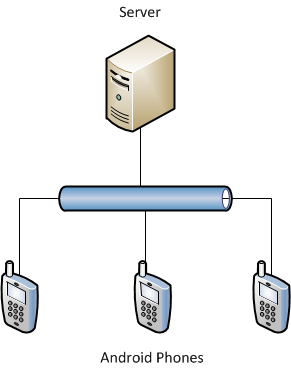
\includegraphics[width=.4\textwidth]{images/design_overview.png}
  \caption{Overview of a standard SnoozZz system}
  \label{fig:images_design_overview}
\end{figure}

% section overview (end)
% chapter design (end)